% \section{Introduction}
% Flat surfaces are pervasive in engineered structures and also occur in natural terrain. For example, structures such as walls, floors, rooftops, and roadways are often flat or ``flat-like". Similarly, home and office furnishings are typically composed of multiple flat surfaces. Sensors such as LiDAR and RGBD cameras generate dense 3D point clouds of these predominately flat surface environments. This observation has been exploited for tasks in localization and mapping \cite{pathak_online_2010},  digital preservation with Photogrammetry and laser scanning \cite{malihi_3d_2016, lerma_terrestrial_2010, balsa-barreiro_generation_2018}, and point cloud registration \cite{rusinkiewicz_efficient_2001}. Planar segmentation techniques are often used to group points together belonging to a flat surface \cite{feng_fast_2014, pham_geometrically_2016-1, schaefer_maximum_2019}. However points clouds are dense incurring a high computational cost when used directly in higher level tasks. Planar point clouds can be converted to lower dimensional representations such as polygons. Polygons reduce map size, accelerate matching for localization \cite{lee_indoor_2012-1}, and support model reconstruction and object detection \cite{cao_roof_2017}. 

% Planar points clouds may be converted to convex polygons \cite{biswas_planar_2012}. Convex polygons are simple and efficient to generate but often do not represent the true shape of a point set. Non-convex polygons may be generated using techniques such as $\alpha$-shapes but operate strictly on 2D data, requiring the projection of each 3D planar point cloud and expensive triangulation \cite{lee_fast_2013, edelsbrunner_shape_1983}. Pixel-level boundary following of organized point clouds can be used to extract non-convex polygons but often only captures the exterior shell of the polygon \cite{lee_indoor_2012-1}. These methods are not able to capture \emph{interior} holes in a polygon representing the shape of obstacles on flat surfaces. Finally, speed is an important consideration for many of the applications mentioned previously. Parallel algorithms written for multi-core CPUs and GPUs should be used to reduce latency. 



This chapter summary presents Polylidar3D, a non-convex polygon extraction algorithm that takes as input either unorganized 3D point clouds (e.g., airborne LiDAR point clouds), organized point clouds (e.g., range images), or user-provided meshes. The non-convex polygons extracted represent flat surfaces in a 3D environment, while interior holes represent obstacles on these surfaces.  Figure \ref{fig:ch3_polylidar_overview} provides an overview of Polylidar3D's data input, front-end, back-end, and output. Currently only one planar direction can be extracted from unorganized 3D point clouds while all other 3D data inputs do not have this limitation. The front-end transforms input data into a half-edge triangular mesh.  This representation provides a common level of abstraction offering increased efficiency for back-end operations. The back-end is composed of four core algorithms: mesh smoothing, dominant plane normal estimation, planar segment extraction, and polygon extraction.  Polylidar3D outputs planar triangular segments, sets of flat connected triangles, and their polygonal representations. Polylidar3D is extremely fast, typically executing in a few milliseconds. It makes use of CPU multi-threading and GPU acceleration when available. 

% Main contribution of this chapter are:

% \begin{itemize}
%   \item An efficient and versatile open source \cite{Castagno_Github_Polylidar} framework for concave (multi)polygon extraction for 3D data. Input can be unorganized/organized 3D point clouds or user-provided meshes.
%   \item A fast open source \cite{Castagno_Github_fastga} dominant plane normal estimation procedure using a Gaussian Accumulator that can also be used as a stand-alone algorithm.
%   \item Multiple diverse open source experiments showing qualitative and quantitative benchmark results from data sources including LiDAR and RGBD cameras \cite{Castagno_Github_Polylidar3D_Kitti, Castagno_Github_Polylidar3D_RealSense, Castagno_Github_Polylidar_Synpeb}.
%   \item Improved half-edge triangulation efficiency for organized point clouds; CPU multi-threaded and GPU accelerated mesh smoothing \cite{Castagno_Github_opf}. 
%   \item Planar segmentation and polygon extraction performed in tandem using task-based parallelism to reduce latency for time-critical applications. 
% \end{itemize}

\begin{figure}[ht]
    \centering
    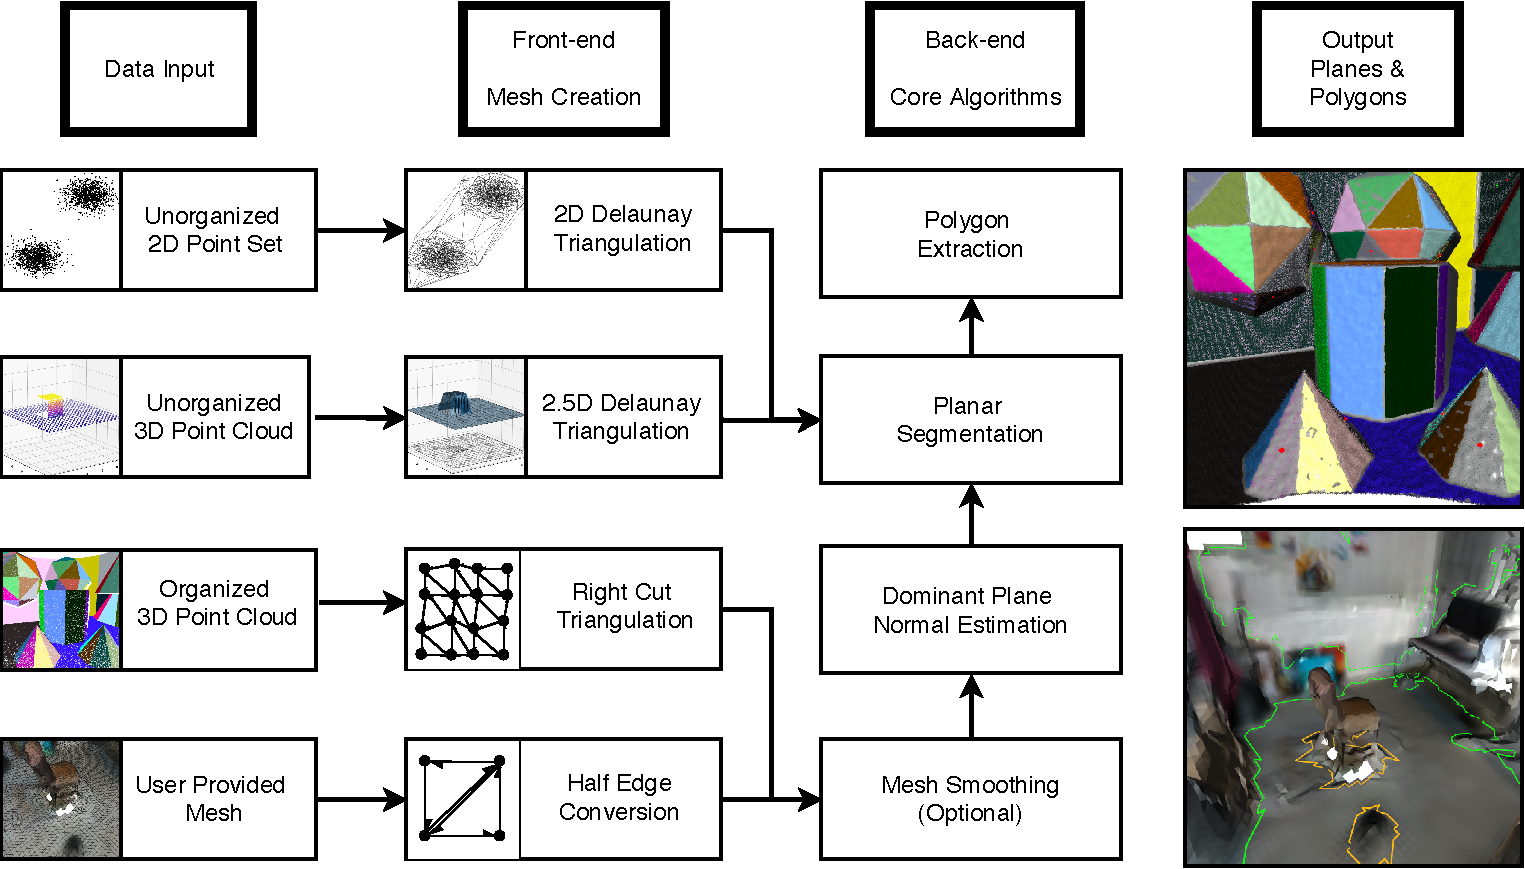
\includegraphics[width=.95\linewidth]{chapter_3_polylidar3d/imgs/Polylidar3DArchitecture-SimplifedV4.pdf}
    \caption{Overview of Polylidar3D. Input data can be 2D point sets, unorganized/organized 3D point clouds, or user-provided meshes. Polylidar3D's front-end transforms input data to a half-edge triangulation structure. The back-end is responsible for mesh smoothing, dominant plane normal estimation, planar segmentation, and polygon extraction. Polylidar3D outputs both planes (sets of spatially connected triangles) and corresponding polygonal representations. An example output of color-coded extracted planes from organized point clouds is shown (top right). An example of extracted polygons from a user-provided mesh is shown (bottom right). The green line represents the concave hull; orange lines show interior holes representing obstacles.} %Note that only one planar direction can be extracted for unorganized 3D point clouds. This is suitable for airborne LiDAR point clouds. }
    \label{fig:ch3_polylidar_overview}
\end{figure}


\paragraph{Framework Highlights}

A key part of Polyidar3D is estimating dominant plane normals within a 3D scene using a novel Gaussian Accumulator, FastGA. A Gaussian Accumulator discretizes the surface of the unit sphere (S2) into individual cells creating ``bins'' of a histogram. Plane normals from a scene are integrated in the accumulator where subsequent peak detection isolates dominant planes. Unlike other methods that partition the sphere in polar coordinates \cite{borrmann_3d_2011, limberger_real-time_2015}, FastGA tessellates the unit sphere with triangles by recursively subdividing the primary faces of an icosahedron. This removes issues with unequal weighting during accumulation, singularities at the poles, and non-equivariant kernels for peak detection.  Recursion level dictates the approximation of the unit sphere. The integration strategy does not rely upon K-D trees but instead uses a global spatial index from space-filling curves followed by local neighborhood search. All data structures are determined at compile time. We unfold the refined icosahedron into a 2D image in a particular way that guarantees equivariant kernels as outlined in \cite{cohen_gauge_2019} . Standard 2D image peak detection is then performed with nearby peaks clustered using agglomerative hierarchical clustering.



\paragraph{Results}

This section summary offers examples of Polylidar3D applied to real-world and synthetic 3D data. Our full paper (and dissertation chapter) shows examples of Polylidar3D applied to unorganized 3D points including airborne LiDAR point clouds and point clouds generated on a moving vehicle.  Additional experiments of organized point clouds including RGBD cameras as well as a challenging synthetic benchmark set are provided. A final analysis of Polylidar3D applied to 3D meshes explores how polygon extraction scales with additional CPU cores. For brevity only the comparison benchmark set is shown. 

% \subsection{SynPEB Benchmark}

Polylidar3D was evaluated on SynPEB, a benchmark dataset used to evaluate plane segmentation algorithms and created by the authors of PPE  \cite{schaefer_maximum_2019}. SynPEB is generated from a room populated with various polyhedra such that each image contains an average of 42.6 planes. LiDAR scans are simulated with different levels of normally-distributed radial and tangential noise producing organized point clouds of size 500 $\times$ 500. There are four levels of tangential noise in the dataset with 0.5 mdeg, 1 mdeg, 2 mdeg, and 4 mdeg standard deviation.  Data is partitioned into a training set to tune algorithm parameters and a test set for evaluation. The combination of high-noise data and numerous small, connected but distinct planes results in challenges for plane segmentation.% as shown in Figure \ref{fig:synpeb_pics}. 
%The noisy color-coded ground truth point cloud is shown in (a), a zoomed-in section of the generated mesh with no smoothing is shown in (b),  our Laplacian and bilateral smoothing is shown in (c), and (d) and (e) show the planes and polygons generated by Polylidar3D. 

Table~\ref{table:synpeb_results} shows benchmark test results (1mdeg of tangential noise) of Polylidar3D against other plane segmentation methods. The~results of other methods including timings are provided in Schaefer et al.~\cite{schaefer_maximum_2019}.  Note that execution times cannot be directly compared but will give an idea of real-time capability. Polylidar3D produces both a point set and polygonal representation of identified planes; however, this benchmark must be evaluated by the point set.   A~``plane'' is considered correctly identified if its point set overlaps with the ground truth plane with the standard 80\% threshold described in Hoover et al.~\cite{hoover_experimental_1996}. Key metrics are $f$ representing the percent of ground truth planes identified, $k$ indicating percent of the point cloud correctly identified, and~RMSE quantifying accuracy of each plane fit. Variables $n_o$, $n_u$, $n_m$, and~$n_s$ represent the absolute numbers of  oversegmented,  undersegmented,  missing,  and~spurious  planes, respectively,  compared  to  the  ground-truth  segmentation. See~\cite{schaefer_maximum_2019,hoover_experimental_1996} for detailed definitions of these metrics. %Red, green, and~yellow blocks in Figure~\ref{fig:synpeb_d} represent missed, spurious, and~oversegmented planes, respectively. 
An $f$ metric of 47.3\% indicates Polylidar3D did not capture most planes in the benchmark, but the $k$ metric of 78.3\% indicates Polylidar3D did well in capturing large dominant planes comprising most of the point cloud.  Additionally there are fewer spurious, over~segmented, and~under segmented planes generated by Polylidar3D than with other methods. Polylidar3D's RMSE value is also lowest, indicating predicted planes have a good fit. Plane segmentation is accomplished in less time, especially in comparison to PPE. Defined $f$ and $k$ metrics indicate PPE does an excellent job of capturing the numerous small planes in the scene but fails slightly more often in capturing large dominant planes.  Polylidar3D uniquely generates concave polygons providing a condensed representation of identified planes. Note polygon generation is included in Polylidar3D timing.





%  Note that RMSE is computed on input noisy point cloud (as all other implementations). 
\begin{table}[H]
\centering
\caption{SynPEB Benchmark~Results.  }
\label{table:synpeb_results}
\begin{tabular}{@{}ccccccccc@{}}
\toprule
\textbf{Method}                                  & $\textbf{f}$ {\textbf{[}}\textbf{\%}{\textbf{]}} & $\textbf{k}$ {\textbf{[}}\textbf{\%}{\textbf{]}} & \textbf{RMSE} {\textbf{[}}\textbf{mm}{\textbf{]}} & $\textbf{n}_\textbf{o}$ & $\textbf{n}_\textbf{u}$ & $\textbf{n}_\textbf{m}$ & $\textbf{n}_\textbf{s}$ & \textbf{time}\\ \midrule
PEAC~\cite{feng_fast_2014}              & 29.1         & 60.4         & 28.6          & 0.7   & 1.0   & 26.7  & 7.4   & \textbf{33 ms}\\
MSAC~\cite{torr_mlesac_2000}            & 7.3          & 35.6         & 34.3          & 0.3   & 1.0   & 36.3  & 10.9  & 1.1 s\\
PPE~\cite{schaefer_maximum_2019}      & \textbf{73.6}         & 77.9         & 14.5          & 1.5   & 1.1   & 7.1   & 16.5  & 1.6 hr\\
Polylidar3D (proposed)                  & 47.3         & \textbf{78.3}         & \textbf{7.2}           & \textbf{0.1}   & \textbf{0.3}   & \textbf{22.8}  & \textbf{4.9}  & 34 ms\\ \bottomrule
\end{tabular}
\end{table}


\paragraph{Conclusion}
This chapter introduced Polylidar3D, a non-convex polygon extraction framework for capturing flat surfaces from a variety of 3D data sources. Polylidar3D has been evaluated in five separate experiments with airborne LiDAR point clouds, automotive LiDAR point clouds, RGBD videos, synthetic LiDAR benchmark data, and meshes of indoor environments. Qualitative and quantitative results demonstrate Polylidar3D's speed and versatility. A complete description of the framework and individual algorithms with additional results is available in \cite{castagno_polylidar3d_2020}.


% Below, Sections \ref{sec:background} and \ref{sec:prelim} provide background and mathematical preliminaries, respectively. Section \ref{sec:methods_mesh_creation} describes Polylidar3D's front-end methods for mesh creation. Section \ref{sec:methods_mesh_smoothing} outlines optional mesh smoothing while Section \ref{sec:methods_fastga} introduces our dominant plane normal estimation algorithm. Section \ref{sec:methods_polylidar} describes plane and polygon extraction with parallelization techniques. Section \ref{sec:methods_polylidar_polygon_filtering} proposes optional post-processing methods to refine and simplify the polygons.  Section \ref{sec:results} provides qualitative results as well as quantitative benchmarks. Sections \ref{sec:discussion} and \ref{sec:conclusion} provide discussion and conclusion, respectively. 